\documentclass{beamer}

\usepackage[ngerman]{babel}
\usepackage{amsmath}

\mode<presentation>
{
    % Include the theme
    \usetheme{rwth}
    \setbeamercovered{transparent = 28}
}

\title{Interaktive Str\"omungssimulation}
\subtitle{\small{Softwareentwicklungspraktikum}}
\author{
  Gruppe 5
}

% Display the table of contents every time a new subsection begins. The parameter is used as the frame title.
\RWTHtoc{Table of contents}

\begin{document}

% Display the title framen
\RWTHtitle
\section{Aufgabenstellung}
  \subsection{Vorstellung}
    
\begin{frame}{Aufgabe}
   Implementierung einer interaktiven echtzeit 2D Str\"omungssimulation von inkompressiblen Fluiden.
	\begin{figure}[H]
		\centering
		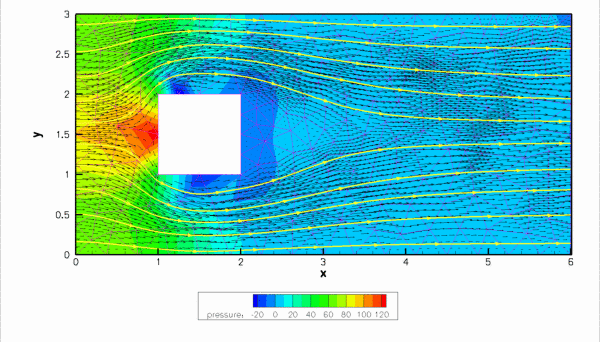
\includegraphics[width= 6.125cm, height = 3.5cm]{box_flow}
		\caption{Str\"omungsbeispiel mit Hindernis}
	\end{figure}
\end{frame}
  
  \subsection{Anforderungen}

\begin{frame}{Bedingungen}
	Implementierung der inkompressiblen Navier-Stokes-Gleichung:
	\begin{itemize}
		\item C++
		\item Benutzeroberfl\"ache mit Qt
		\item Visualisierung mit OpenGL
		\item Echtzeitf\"ahige Randbedingungs\"anderung (z.B Hindernisse einzeichnen, Viskosit\"at \"andern)
		\item Verwendung verschiedener nummerischer Methoden
    \begin{itemize}
    \item Achtung: numerische Stabilit\"at
 	  \end{itemize}
 	  \item Lauff\"ahig auf dem RWTH-Cluster
    \item Minimale Hardware-Anforderungen
	\end{itemize}
\end{frame}
    
  \subsection{Anwendungsfalldiagramm}
    
\begin{frame}{Anwendungsfalldiagramm}
  \begin{figure}[H]
	  \centering
	  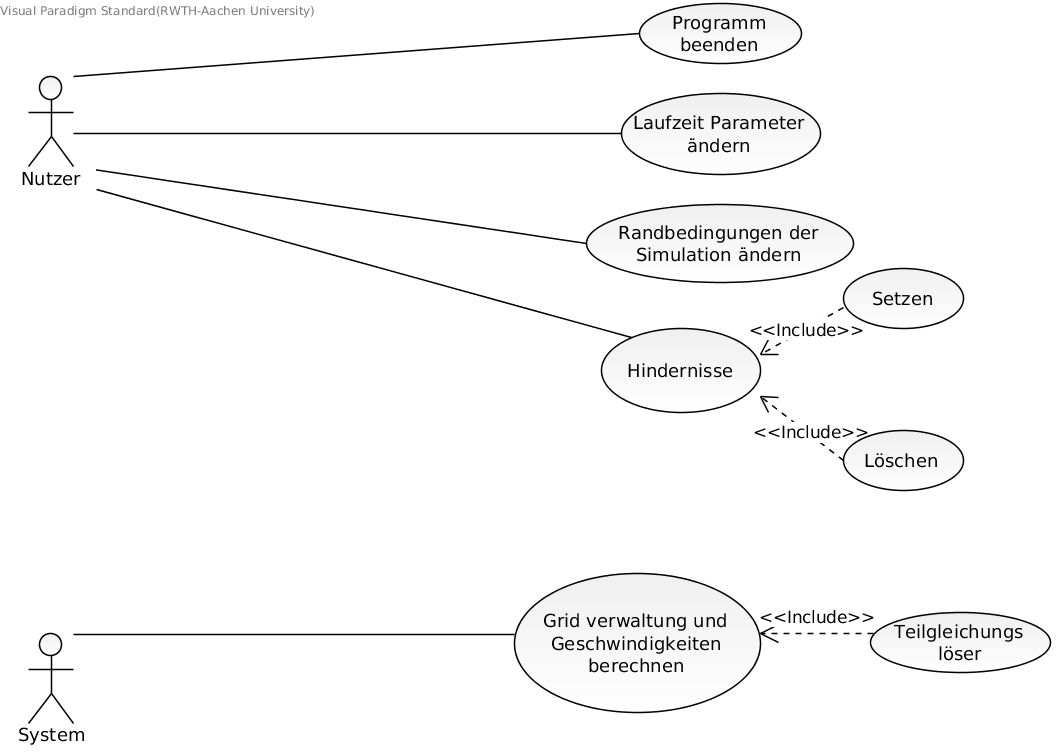
\includegraphics[width=6.49cm,height=5.63cm]{images/Strom-UCD}
	  \caption{Anwendungsfalldiagramm}
  \end{figure}
\end{frame}
  
\section{Mathematik}
  \subsection{Allgemein}

\begin{frame}{Navier-Stokes-Gleichung}
	\begin{align*}
	  \bigtriangledown \cdot \mathbf{u} &= 0
	  \\
	  \frac{\partial \mathbf{u}}{\partial t} &= - \left( \mathbf{u} \cdot \bigtriangledown \right) \mathbf{u} - \frac{1}{\rho} \bigtriangledown p + \nu \bigtriangledown^2 \mathbf{u} + \mathbf{f}
	\end{align*}

	\begin{itemize}
		\item \"Ubliches Diskretisieren mit FDM f\"uhrt bei gro{\ss}en Zeitschritten zu Instabilit\"at
			\begin{itemize}
			\item CFL-Zahl
			\end{itemize}
		\item Ansatz: Semi-Lagrangian scheme
	\end{itemize}
\end{frame}

\begin{frame}{Bedingungen}
	\begin{itemize}
	  \item Gestaffelt kartesisches Gitter
	  \item Verschiedene numerische Methoden
		\begin{itemize}
		\item Bedingungslose Stabilit\"at
		\end{itemize}
  \end{itemize}
\end{frame}

\begin{frame}{Gestaffelt kartesisches Gitter}
	\begin{itemize}
	  \item Vier Geschwindigkeiten
	  \item Ein Vektor mit Parametern
  \end{itemize}
    \begin{figure}[H]
	  \centering
	  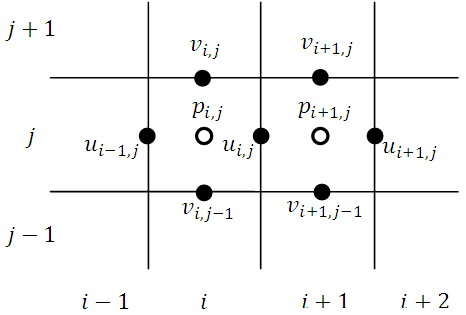
\includegraphics[width=6.49cm]{images/grid}
	  \caption{Gestaffelt kartesisches Gitter}
  \end{figure}
\end{frame}

 \subsection{Navier-Stokes-Gleichung}
\begin{frame}{Navier-Stokes Teilgleichungen}
	Konvektionsterm mit Semi-Lagrangian scheme:
	\begin{align*}
	  \frac{\partial \mathbf{u}}{\partial t} &= \underbrace{\textcolor{red}{- \left( \mathbf{u} \cdot \bigtriangledown \right) \mathbf{u}}}_{\substack{Konvektion}} - \frac{1}{\rho} \bigtriangledown p + \nu \bigtriangledown^2 \mathbf{u} + \mathbf{f}
	\end{align*}
	\begin{itemize}
	\item  Particle Tracer (expliziter Euler oder Runge Kutta):
	\begin{itemize}
	\item  Bei jedem Zeitschritt: Berechne Ursprungspositionen aller Partikel.
	\end{itemize}
	\item Interpolation:
	\begin{itemize}
	\item Approximiert umliegende Gitterpunktwerte aller Partikel an dessen Ursprungspositionen.
	\end{itemize}
	\end{itemize}
\end{frame}

\begin{frame}{Navier-Stokes Teilgleichungen}
	Innere Kr\"afte durch Druck:
	\begin{align*}
	  \frac{\partial \mathbf{u}}{\partial t} &= - \left( \mathbf{u} \cdot \bigtriangledown \right) \mathbf{u} \underbrace{\textcolor{red}{- \frac{1}{\rho} \bigtriangledown p}}_{\substack{Druck}} + \nu \bigtriangledown^2 \mathbf{u} + \mathbf{f}
	\end{align*}
	\begin{itemize}
	\item  Lineares Verfahren, z.B Gauss Seidel
	\end{itemize}
\end{frame}

\begin{frame}{Navier-Stokes Teilgleichungen}
	Diffusionsterm:
	\begin{align*}
 	 \frac{\partial \mathbf{u}}{\partial t} &= - \left( \mathbf{u} \cdot \bigtriangledown \right) \mathbf{u} - \frac{1}{\rho} \bigtriangledown p + \underbrace{\textcolor{red}{\nu \bigtriangledown^2 \mathbf{u}}}_{\substack{Diffusion}} + \mathbf{f}
	\end{align*}
	\begin{itemize}
	\item  Implizites Euler Verfahren
	\end{itemize}
\end{frame}

\begin{frame}{Navier-Stokes Teilgleichungen}
	\"Aussere Kr\"afte:
	\begin{align*}
 	 \frac{\partial \mathbf{u}}{\partial t} &= - \left( \mathbf{u} \cdot \bigtriangledown \right) \mathbf{u} - \frac{1}{\rho} \bigtriangledown p + \nu \bigtriangledown^2 \mathbf{u} + \underbrace{\textcolor{red}{\mathbf{f}}}_{\substack{Kraft}}
	\end{align*}
	\begin{itemize}
	\item  Explizites Euler Verfahren
	\end{itemize}
\end{frame}


\section{Implementation}
  \subsection{Biblotheken}
  \begin{frame}{M\"oglichkeiten}
  \begin{block}{Entschieden}
    \begin{itemize}
      \item Mathematik: \textit{Eigen}
      \item Benutzeroberfl\"ache: \textit{QT 5.5 (wenn m\"oglich sonst 5.*)} 
      \item Eigentliche Str\"omung: \textit{OpenGl eingebettet in Qt}
    \end{itemize}
  \end{block}
  \begin{block}{Unentschlossen}
    \begin{itemize}
      \item Numerischeverfahren: \textit{odeint}
    \end{itemize}
  \end{block}
    \end{frame}
  \subsection{Aufteilung}
    \begin{frame}{Bibliothek, MVC}
    
  \begin{block}{Aufteilung}
    \begin{itemize}
      \item Benutzeroberfl\"ache: Model-View-Controller (MVC) (kein zusammen klicken)
      \item Solver: Reines C++ ohne Qt
    \end{itemize}
    \end{block}
    \begin{block}{Reihenfolge}
     \begin{itemize}
      \item Implimentierung von geg. Code und kartesischen Gitter
      \item \"Ubertragung auf Gestaffelten kartesischen Gitter
    \end{itemize}
    \end{block}
    
    \end{frame}
    \subsection{Demo}
    \begin{frame}{Demo}
      \center \Huge{Demo}
    \end{frame}

  
% \section{Examples}
%
%     \subsection{Subsection 1}
%
%         \begin{frame}{Test}
%             \begin{itemize}
%                 \item Test1
%                 \pause
%                 \item Test1
%                 \pause
%                 \item Test1
%             \end{itemize}
%         \end{frame}
%
%     \subsection{Subsection 2}
%
%         \begin{frame}{Test 2}
%             \begin{block}{Definition}
%                 Lorem ipsum dolor sit amet, consetetur sadipscing elitr, sed diam nonumy eirmod tempor invidunt ut labore et dolore magna aliquyam erat, sed diam voluptua. At vero eos et accusam et justo duo dolores et ea.
%             \end{block}
%         \end{frame}
%
%         \begin{frame}
%             \frametitle{Test 3}
%             \begin{block}{Definition}
%             \begin{itemize}
%                 \item Test1
%                 \item Test1
%                 \item Test1
%             \end{itemize}
%             \end{block}
%         \end{frame}
%
%    \subsection{Subsection 3}
%    
%         \begin{frame}{Test 2}
%        	    Lorem ipsum dolor sit amet, consetetur sadipscing elitr, sed diam nonumy eirmod tempor invidunt ut labore et dolore magna aliquyam erat, sed diam voluptua. At vero eos et accusam et justo duo dolores et ea.
%
%             \begin{align}
%                 R(\alpha) = \int \frac{1}{2} |y - f(x;\alpha)| dP(x,y) \leq R_{emp}(\alpha) + \epsilon(N, \delta, h)
%             \end{align}   
%         \end{frame}
%
%    
%         \begin{frame}{Test 2}
%                 Lorem ipsum dolor sit amet, consetetur sadipscing elitr, sed diam nonumy eirmod tempor invidunt ut labore et dolore magna aliquyam erat, sed diam voluptua. At vero eos et accusam et justo duo dolores et ea.
%             \begin{block}{Definition}
%                 Lorem ipsum dolor sit amet, consetetur sadipscing elitr, sed diam nonumy eirmod tempor invidunt ut labore et dolore magna aliquyam erat, sed diam voluptua. At vero eos et accusam et justo duo dolores et ea.
%             \end{block}
%             \pause
%             \begin{block}{Definition}
%                 Lorem ipsum dolor sit amet, consetetur sadipscing elitr, sed diam nonumy eirmod tempor invidunt ut labore et dolore magna aliquyam erat, sed diam voluptua. At vero eos et accusam et justo duo dolores et ea.
%             \end{block}
%         \end{frame}
%
%         \begin{frame}{Test 3}
%             \begin{block}{Normal block}
%             block text
%             \end{block}
%             
%             \begin{exampleblock}{Example block}
%             block text
%             \end{exampleblock}
%             
%             
%             \begin{alertblock}{Alert block}
%             block text
%             \end{alertblock}
%         \end{frame}
%
%         \begin{frame}{Test 4}
%             \begin{theorem}
%             block text
%             \end{theorem}
%             
%             \begin{proof}
%             block text
%             \end{proof}
%
%         \end{frame}
%
%
%         \begin{frame}{Test 5}
%
%             \begin{tabular}{|c|c|c|}
%             \hline
%             \textbf{Test0} & \textbf{Test1} & \textbf{Test2} \\
%             \hline
%             Test1 & Test2 & Test3 \LaTeX  \\
%             \hline
%             Test4 & Test5& Test6\\
%             \hline
%             \end{tabular}
%             
%         \end{frame}
%
%         \begin{frame}{Test 6}
%
%             \begin{exampleblock}{Example block}
%                 \smallskip 
%
%                 \begin{tabular}{|c|c|c|}
%                 \hline
%                 \textbf{Test0} & \textbf{Test1} & \textbf{Test2} \\
%                 \hline
%                 Test1 & Test2 & Test3 \LaTeX  \\
%                 \hline
%                 Test4 & Test5& Test6\\
%                 \hline
%                 \end{tabular}
%             \end{exampleblock}
%
%             \begin{block}{Block}
%                 \smallskip 
%
%                 \begin{tabular}{|c|c|c|}
%                 \hline
%                 \textbf{Test0} & \textbf{Test1} & \textbf{Test2} \\
%                 \hline
%                 Test1 & Test2 & Test3 \LaTeX  \\
%                 \hline
%                 Test4 & Test5& Test6\\
%                 \hline
%                 \end{tabular}
%             \end{block}
%         \end{frame}
%
% 	 \begin{frame}{Test 7}
%             
%          	\begin{block}{Block A}
%             
%                 \begin{description}[longest label]
%                     \item[short] Short stuff
%                     \item[long] Longer stuff
%                     \item[longest label] Longest stuff (insert cat)
%                 \end{description}
%             
%                 \begin{itemize}
%                     \item item1
%                     \item item2
%                     \item item3
%                 \end{itemize}  
%             \end{block}
%
%         \end{frame}
%
%         \begin{frame}[t]{Frame with Columns}
%             \begin{columns}[t]
%                 \column{0.4\textwidth}
%
%                 \begin{block}{Block 1}
%                     Text here
%                 \end{block}
%
%                 \column{0.4\textwidth}
%
%                 \begin{block}{Block 2}
%                     More text here
%                 \end{block}
%             \end{columns}
%         \end{frame}
%
%         \begin{frame}[t]{Frame without Columns}
%             \leavevmode
%             \begin{block}{Block}
%                 Even more text here
%             \end{block}
%         \end{frame}
\end{document}
